\documentclass[tikz]{standalone}
\usepackage{fontspec}
\renewcommand*{\familydefault}{\sfdefault}
\usepackage{standalone}
\usepackage{amssymb}
\usetikzlibrary{decorations}
\usetikzlibrary{arrows.meta, decorations.pathmorphing, decorations.pathreplacing, shapes.geometric}
\usetikzlibrary{bayesnet}

\begin{document}

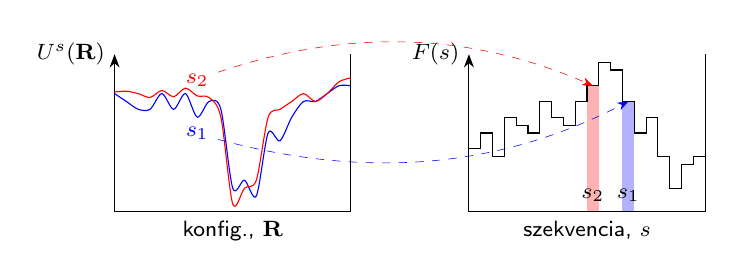
\begin{tikzpicture}[font=\footnotesize, xscale=1.5]

% axes
\draw[-Stealth] (-1,0) -- (-1,2) node[anchor=east] {\(U^s(\mathbf{R})\)} ;
\draw (1,0) -- (1,2) ;
\draw (-1,0) -- node[anchor=north] {konfig.,~\(\mathbf{R}\)} (1,0) ;

% energy landscape
\draw[blue] plot[smooth] coordinates {
(-1.0,1.5) (-0.9,1.4) (-0.8,1.3) (-0.7,1.3) (-0.6,1.5) (-0.5,1.3) (-0.4,1.5)
(-0.3,1.2) (-0.2,1.4) (-0.1,1.3) (0.0,0.3) (0.1,0.4) (0.2,0.2) (0.3,1.0) (0.4,0.9) (0.5,1.2) (0.6,1.4) (0.7,1.4) (0.8,1.5) (0.9,1.6) (1.0,1.6)
};

% energy landscape
\draw[red] plot[smooth] coordinates {
(-1.0,1.52) (-0.9,1.53) (-0.8,1.5) (-0.7,1.45) (-0.6,1.54) (-0.5,1.46)
(-0.4,1.57)
(-0.3,1.47) (-0.2,1.45) (-0.1,1.2) (0.0,0.1) (0.1,0.3) (0.2,0.4) (0.3,1.2)
(0.4,1.3) (0.5,1.4) (0.6,1.5) (0.7,1.4) (0.8,1.5) (0.9,1.65) (1.0,1.7)
};

% landscape labels
\node[anchor=north, blue] at (-0.3,1.2) (Us1) {\(s_1\)};
\node[anchor=south, red] at (-0.3,1.47) (Us2) {\(s_2\)};

% fitness landscape
\begin{scope}[xshift=3 cm]

% color bars for F(s1) and F(s2)
\fill[blue!30!white] (0.3,0) rectangle (0.4,1.4) ;
\fill[red!30!white] (0,0) rectangle (0.1,1.6) ;

% labels for s1 and s2
\path
(0.35,0) node[anchor=south] {\(s_1\)}
(0.05,0) node[anchor=south] {\(s_2\)}
;

% axes
\draw[-Stealth] (-1,0) -- (-1,2) node[anchor=east] {\(F(s)\)} ;
\draw (1,0) -- (1,2) ;
\draw (-1,0) -- node[anchor=north] {szekvencia, \(s\)} (1,0) (1,0) ;

% landscape
\draw[black] plot[const plot] coordinates {
(-1.0,0.8) (-0.9,1.0) (-0.8,0.7) (-0.7,1.2) (-0.6,1.1) (-0.5,1.0) (-0.4,1.4) (-0.3,1.2) (-0.2,1.1) (-0.1,1.4) (0.0,1.6) (0.1,1.9) (0.2,1.8) (0.3,1.4) (0.4,1.0) (0.5,1.2) (0.6,0.7) (0.7,0.3) (0.8,0.6) (0.9,0.7) (1.0,0.7)
};

% energy to fitness mappings
\begin{scope}[-Stealth, dashed, very thin]
\draw[blue] (Us1) to[bend right] (0.35,1.4) ;
\draw[red] (Us2) to[bend left] (0.05,1.6) ;

\end{scope}

\end{scope}

\end{tikzpicture}

\end{document}
